\chapter{Implementation}

\section{Introduction}
This chapter will explore the final implementation of the proposed system. It will give an overview of the final system as well as discuss the languages and libraries used. It will also highlight the issues that were encountered during the development process. Furthermore, it will discuss the comparison system used in the final usability evaluation and the maintainability of each of the systems.

\section{System Overview}
As shown in Figure \ref{fig:componentDiagram}, the final system was separated into two individual systems: a scripting tool and a web application. The scripting tool generates the required files for the web application based on information from Bioschemas and Schema.org. The web application then uses these files to display a form and additional information to allow users to markup Bioschemas profiles.

Separating the file generation from the web application allowed the load times to be kept as low as possible. By generating the files separately and having the web application fetch the generated files, it removes the time needed for the web application to generate the files each time the application is loaded.


\newpage
\vspace*{2em}
\begin{figure}[!h]
 \centering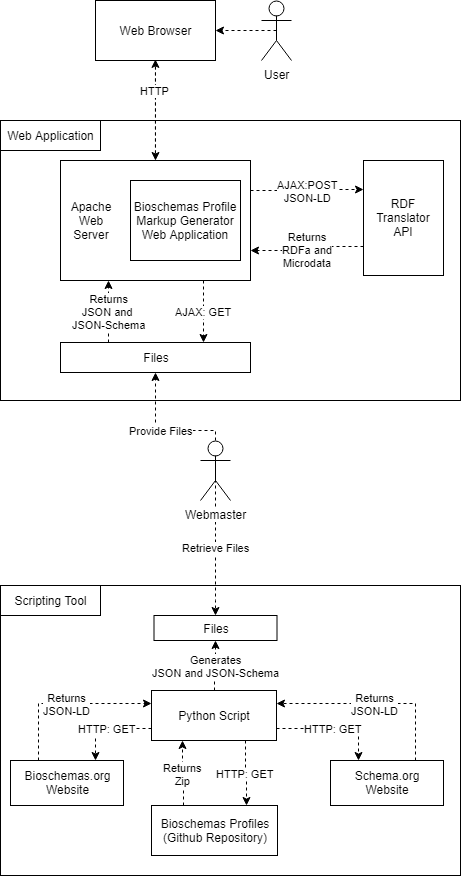
\includegraphics[scale=0.6]{images/ComponentDiagram.png}
   \caption{Component Diagram}
   \label{fig:componentDiagram}
\end{figure}

\newpage
\section{Scripting Tool}\label{sec:scriptingtool}

\subsection{Choice of Language}
After developing the initial prototype to help gather requirements and ensuring I was happy with the approach to utilise JSON-Schema to generate the form. The next step was to begin developing a tool that takes the declarative descriptions of the Bioschemas profiles and generates the required files (JSON and JSON-Schema).

To implement this tool, I had two different options available. I could either extend the Bioschemas GoWeb tool which generates the declarative description of the Bioschemas Profiles or create a separate tool in Python that takes the output of GoWeb and further processes it.

\subsubsection{Bioschemas GoWeb}
Go\footnote{\url{https://golang.org} (accessed 28/02/2019)}, also known as GoLang, is an open source language developed by Google that is similarly modelled after C \cite{goLang} and is also considered to be lightly object-orientated \cite{goObject}. While I do not have any experience with this language specifically, I have a lot of experience working with object-orientated languages but have very limited experience with C. 

Bioschemas GoWeb\footnote{\url{https://github.com/BioSchemas/bioschemas-goweb} (accessed 28/02/2019)}, developed in Go, is a tool that generates a declarative description of the Bioschemas profiles. The declarative descriptions that it generates is a human friendly but machine readable format called YAML\footnote{\url{https://yaml.org/} (accessed 28/02/2019)}. To generate the YAML, the tool uses CSVs which contains information about the Bioschemas profiles. To aid the webmasters in creating the CSVs, a Google Sheets template and detailed instructions are provided.

This is a valid option for our scripting tool as we could extend Bioschemas GoWeb by taking the YAML it produces and then generating the files needed directly from it. Furthermore, by generating the files directly from the YAML, it mitigates the need to retrieve the generated YAML from the Bioschemas Github\footnote{\url{https://github.com/BioSchemas/bioschemas.github.io} (accessed 28/02/2019)}.

\subsubsection{Python Tool}
Python\footnote{\url{https://python.org} (accessed 28/02/2019)} is a object-orientated language, high-level programming language that is often used for rapid prototyping. Through university coursework and personal projects I have a lot of experience with this language as well as other object-orientated languages. 

This is a valid option as the YAML generated by the GoWeb tool for the Bioschemas profiles is available through the Bioschemas Github. In this case we would be able to retrieve the YAML directly from the Github and then further process the YAML into the desired files, instead of processing the CSV's directly to generate the YAML first like in the GoWeb tool.

\subsubsection{Selection}
While the Bioschemas GoWeb tool is a good starting point in developing this tool, I can not neglect my experience and knowledge with Python and object-orientated programming. Also as time management is critical in this project, with Python having a more extensive selection of libraries and being utilised in rapid prototype development, the tool will be written in Python. 

\subsection{Declarative Description Processing}\label{sec:declarative}
The first stage of generating the required files for the web application was retrieving information about and surrounding the Bioschemas profiles and converting it into a usable format. As the information is collected from multiple sources (Shown in Figure \ref{fig:componentDiagram}), two methods of retrieval and conversion were used. 

For the first method, the information about the Bioschemas profiles were located on the Bioschemas Github and were in the YAML format. Using Python library Requests\footnote{\url{http://docs.python-requests.org/en/master/} (accessed 28/02/2019)} the YAML was retrieved using HTTP GET requests. The Python library PyYAML\footnote{\url{https://pyyaml.org/} (accessed 28/02/2019)} was then used to convert the YAML into a Python object to be further processed. Shown in Appendix \ref{sec:geneYAML} is an example of the YAML retrieved for the Bioschemas profile Gene\footnote{\url{https://bioschemas.org/specifications/Gene/} (accessed 28/02/2019)} and the resulting Python object displayed as JSON is shown in Appendix \ref{sec:genePythonObject}.

\newpage
The second method was used to fetch additional information about Bioschemas and Schema.org types. Similar to the first method, this was achieved  using the Request Python library to perform HTTP GET requests to retrieve the information in the format of JSON-LD. As JSON-LD only adds specific key pair values in comparison to JSON, I was able to use the Python library JSON\footnote{\url{https://docs.python.org/2/library/json.html} (accessed 28/02/2019)} to convert the JSON-LD into a Python object to be further processed. Shown in Appendix \ref{sec:BioChemJSONLD} is the JSON-LD for the Bioschemas type BioChemEntity\footnote{\url{http://bio.sdo-bioschemas-227516.appspot.com/BioChemEntity} (accessed 05/04/2019)}.

Once the methods of retrieving the information was figured out, the next stage of the process was to generate the JSON-Schema\footnote{\url{https://json-schema.org/} (accessed 05/04/2019)} used to display the form on the web application. To create the JSON-Schema, I was able to create a Python dictionary of key value pairs and then using the JSON library I was able to output the dictionary as JSON-Schema. During this stage, I encountered three major issues that are discussed in Section \ref{sec:issues}. Through using the iterative development process and help from my supervisor Dr. Alasdair Gray, I was able to work through these issues to create the JSON-Schema describing the Bioschemas profiles. Shown in Appendix \ref{sec:geneJSONSchema} is an example of the JSON-Schema generated for the Bioschemas Gene profile.

The final stage of the process was to generate JSON that is used to display additional information (examples and controlled vocabulary) along side the form on the web application. This used the same method as creating the JSON-Schema, by creating a Python dictionary of key value pairs and then utilising the Python library JSON to output the dictionary as JSON. Shown in Appendix \ref{sec:geneAdditionalInformation} is example of the generated JSON for the Bioschemas Gene profile.

To summarise, the scripting tool generates two files for each Bioschemas profile: A JSON-Schema file that is used by the JavaScript library JSON-Editor (See Section \ref{sec:jsoneditor}) to display a form that the user can use to provide data to markup Bioschemas profiles and a JSON file that contains the controlled vocabularies and examples of the profiles properties to be displayed along side the form (See Section \ref{sec:additionalinformation}).


\newpage
{\setstretch{1.85}
\section{Web Application}\label{sec:webapplication}
The web application consists of an Apache Web Server\footnote{\url{https://httpd.apache.org/} (accessed 12/03/2019)} (Version 2.2.15), containing the front-end user interface as well as JavaScript scripts and libraries for client-side processing. The web application retrieves the generated files from the scripting tool (See Section \ref{sec:declarative}) from the Apache Web Server and using a multitude of libraries (See Section \ref{sec:libraries}), provides the desired functionality of the proposed system. 

\subsection{User Interface Design}\label{sec:userInterface}
The user interface provides an easy and intuitive way for users to select, provide information and generate the markup for a Bioschemas profile. It was developed using HTML5, CSS3 and Bootstrap 4. I used Bootstrap\footnote{\url{https://getbootstrap.com/} (accessed 12/03/2019)} as a front-end web framework to handle the layout, styling and fonts of the HTML elements that are displayed to the user. Bootstrap also supports the latest, stable releases of all major browsers and platforms, which forms part of the system requirements (Non-Functional Requirement NFR3: The system should be accessible through the top internet browsers: Google Chrome, Mozilla Firefox and Apple Safari.).

\subsubsection*{Select Profile}
The Select Profile section is designed to allow users to select which Bioschemas profile they would like to generate a markup for through a drop-down list, shown in Figure \ref{fig:selectProfle}. Unfortunately, as the profiles are added to the drop-down list asynchronously, the resulting drop-down list is not alphabetically ordered, possibly adding time for a user to find their desired profile. The "Generate Form" button then displays the form for the Bioschemas profile they selected.\newline

\begin{figure}[!h]
 \centering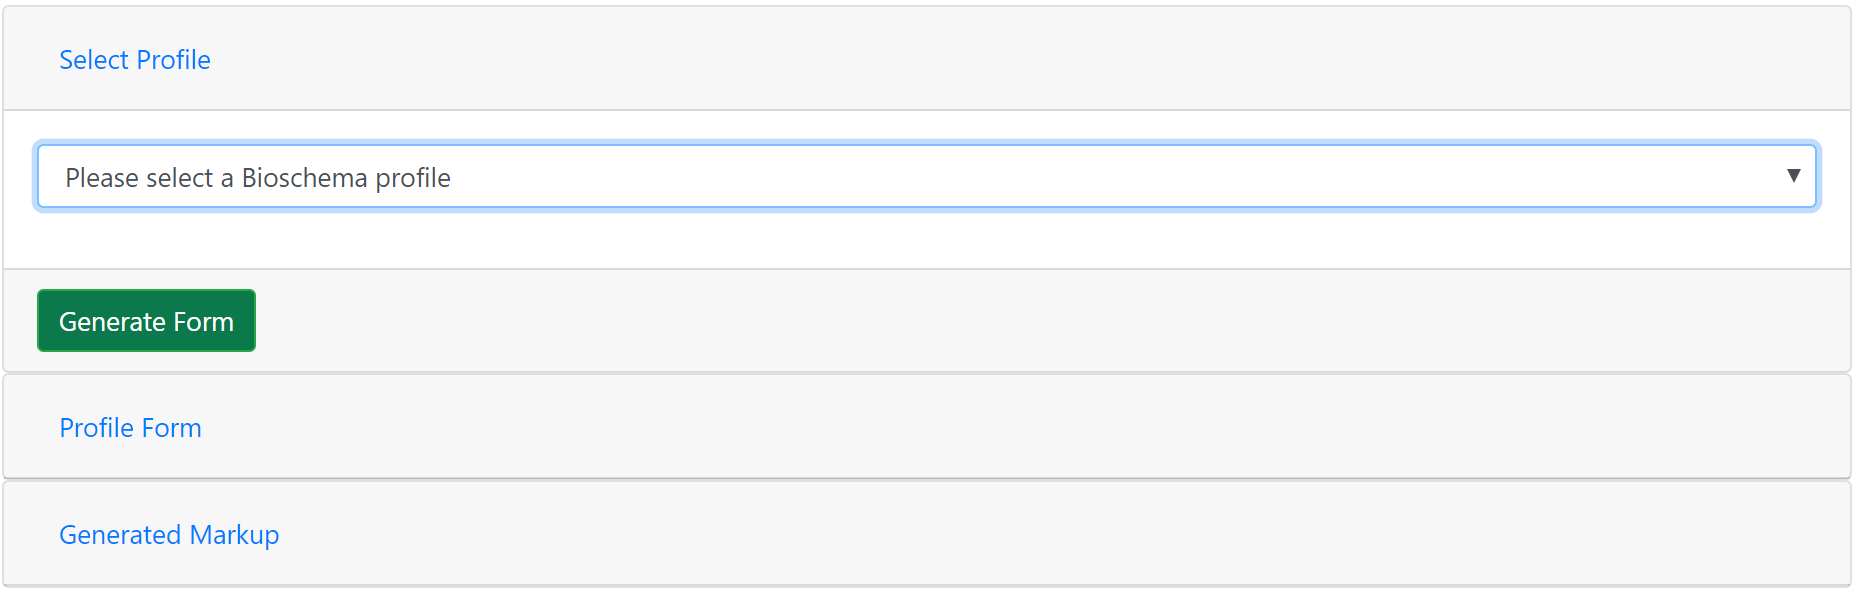
\includegraphics[scale=0.65]{images/system/generateForm.PNG}
   \caption{Select Profile}
   \label{fig:selectProfle}
\end{figure}

}

\newpage
\subsubsection*{Profile Form}
The Profile Form section is designed to allow the user to provide information to markup a Bioschemas profile they previously selected, shown in Figure \ref{fig:geneProfile}. The page is designed as two parts: the left hand side displaying the form for users to provide the information with the right hand side providing additional information like examples and controlled vocabularies. \newline

\begin{figure}[!h]
 \centering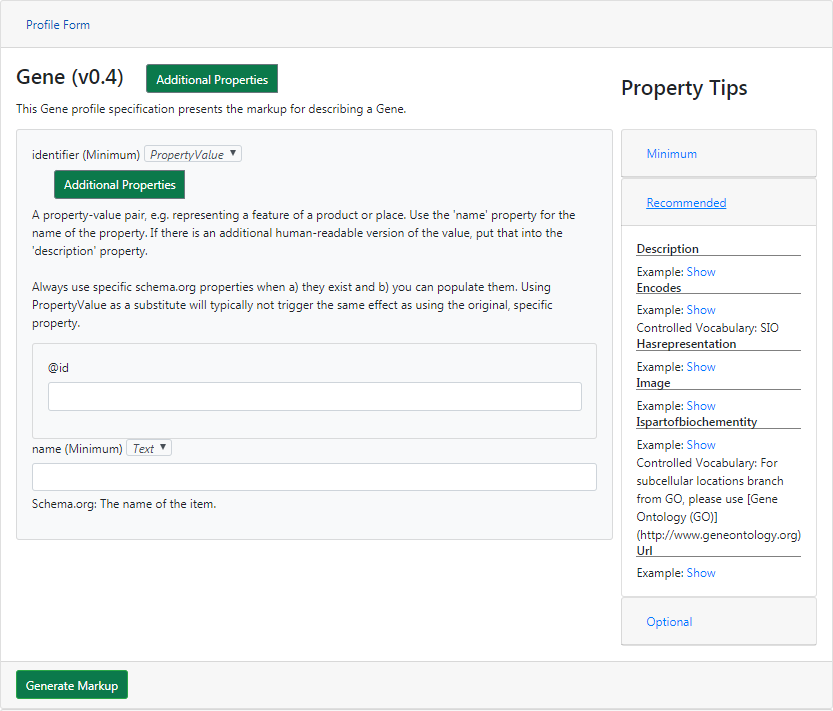
\includegraphics[scale=0.7]{images/system/geneForm.PNG}
   \caption{Bioschemas Profile Gene Form}
   \label{fig:geneProfile}
\end{figure}

\newpage
The form is displayed using the JSON-Editor JavaScript library, which will be discussed in Section \ref{sec:jsoneditor} and is styled using Boostrap 4. By default it displays the Minimum required properties of the Bioschemas Profile. To add the Recommended and Optional properties to the form, select the "Additional Properties" button, shown in Figure \ref{fig:additionalProperties} and then select the check box next to the desired properties.\newline

\begin{figure}[!h]
 \centering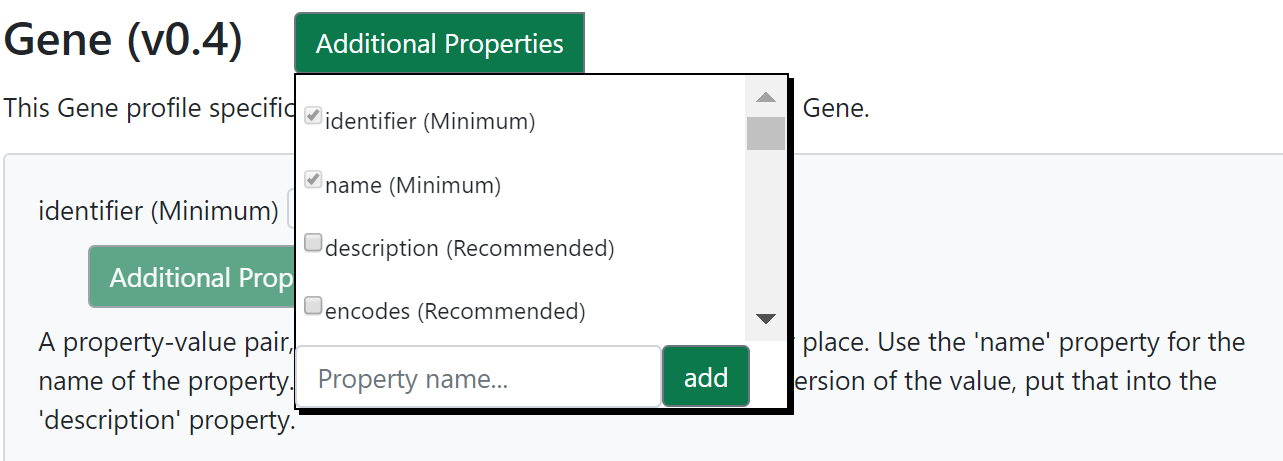
\includegraphics[scale=0.7]{images/system/geneAdditionalProperties.PNG}
   \caption{Bioschemas Profile Gene Additional Properties}
   \label{fig:additionalProperties}
\end{figure} 

For Properties that have a cardinality of many, items can be added through the "Add item" button shown in Figure \ref{fig:arrayAdd}. Once an item has been added, the type of item can then be selected through the drop-down, the example shown in \ref{fig:arrayDelete} is of type URL\footnote{\url{https://schema.org/URL} (accessed 12/03/2019)}. To remove an item, select the "Delete item" button and then confirm through the browser pop-up.

\begin{figure}[!h]
 \centering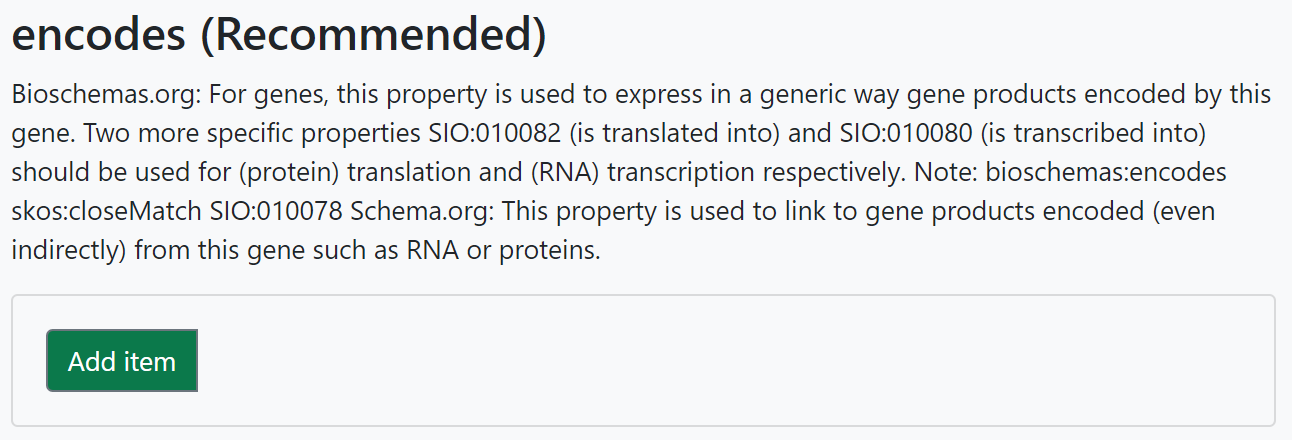
\includegraphics[scale=0.8]{images/system/geneAdd.PNG}
   \caption{Bioschemas Profile Gene Encodes Array}
   \label{fig:arrayAdd}
\end{figure}

\begin{figure}[!h]
 \centering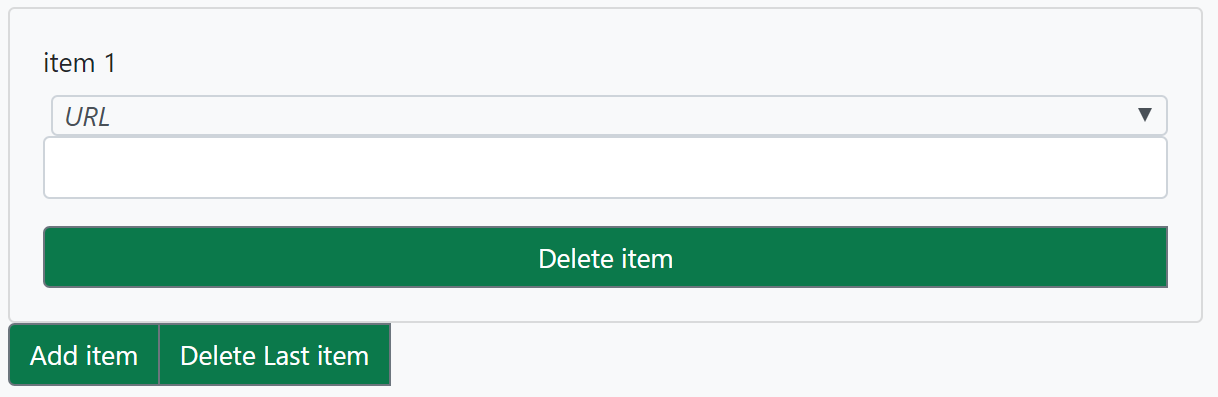
\includegraphics[scale=0.8]{images/system/geneRemove.PNG}
   \caption{Bioschemas Profile Gene Encodes Array Item}
   \label{fig:arrayDelete}
\end{figure}

{\setstretch{1.7}
\newpage
The Property Tips are displayed using a custom script, see Section \ref{sec:additionalinformation} and is styled using Bootstrap 4. I decided to split the additional information into three collapsible sections, by marginality of the properties (Minimum, Recommended and Optional). Taking inspiration from the Bioschemas website, I decided that the best way to display the examples to the user was to use a modal pop-up, shown in Figure \ref{fig:geneEncodesExample}. The decision to separate and nest the additional information was taken to reduce the information overload to the user and to hopefully not confuse them straight away.\newline

\begin{figure}[!h]
 \centering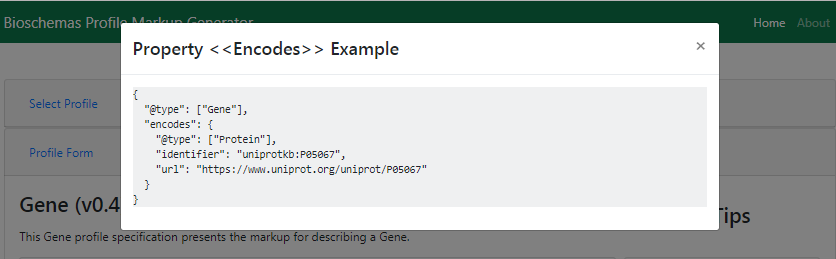
\includegraphics[scale=0.45]{images/system/propertyExample.PNG}
   \caption{Bioschemas Profile Gene Encodes Example}
   \label{fig:geneEncodesExample}
\end{figure}

\subsubsection*{Generated Markup}
The Generated Markup section shows the user the generated markup based on the Bioschemas profile they selected and the information they provided, shown in Figure \ref{fig:generatedMarkup}. The web application generates three formats of machine-readable data: JSON-LD, Microdata and RDFa, which can be accessed through the appropriate navigation tabs. The "Download" button also allows the user to download the generated markup (which ever format is currently being displayed) into a HTML file.\newline

\begin{figure}[!h]
 \centering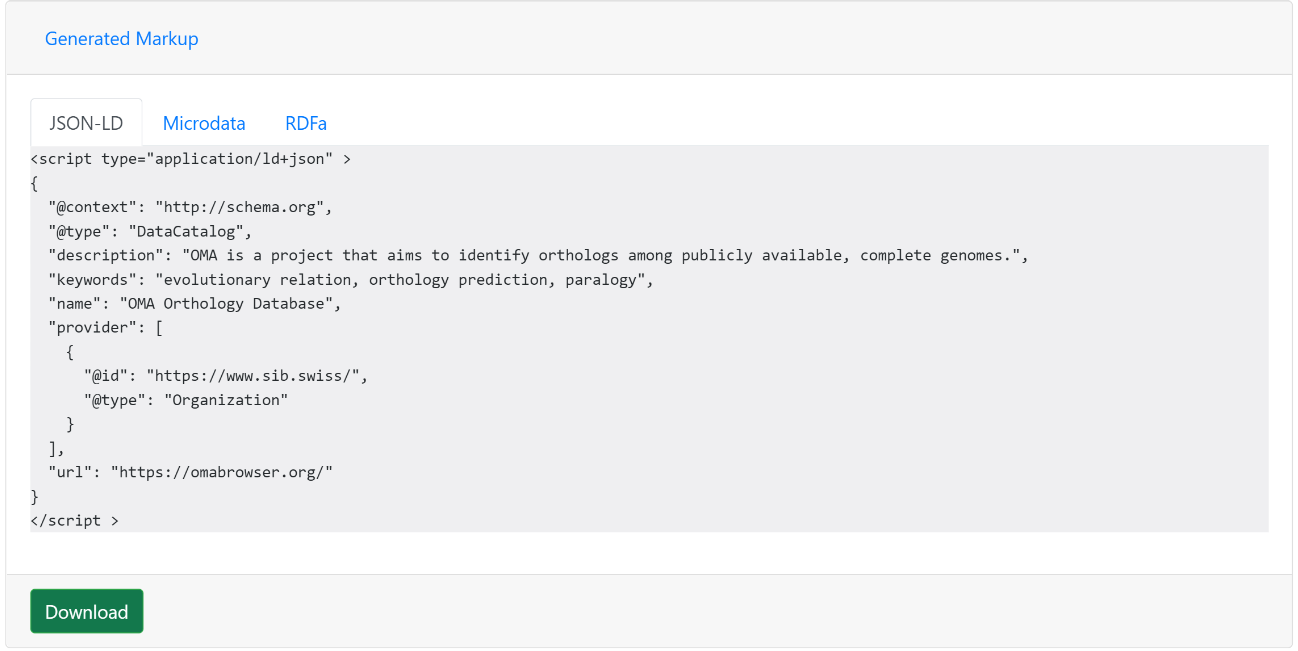
\includegraphics[scale=0.39]{images/system/GeneratedData.PNG}
   \caption{Bioschemas Profile Markup DataCatalog Example}
   \label{fig:generatedMarkup}
\end{figure}

}

\newpage
\subsection{Scripts, Libraries and APIs}\label{sec:libraries}

\subsubsection{JSON-Editor} \label{sec:jsoneditor}
To dynamically generate the forms for the Bioschemas profiles 


The approach I decided was best to dynamically create the forms for the Bioschemas profiles was to utilise JSON-Schema. 


The JSON-Schema is generated by the scripting tool (See Section \ref{sec:scriptingtool}) and using a library the JSON-Schema is displayed as a form. Through the iterative design cycle, three libraries were used as requirements and limitations of the different libraries came to light. I will now discuss the first two libraries used in the prototype system in comparison to the library used in the final system.

The prototype system had two development iterations. The first iteration, was built using SchemaForm.io\footnote{\url{http://www.schemaform.io/} (accessed 03/11/2018)}. As mention in the prototyping Section \ref{ch:prototyping}, I quickly discovered that the library was inadequate for this system due not being able to support JSON arrays of multiple types. why is this a problem?


The second iteration was built using JSON-Forms\footnote{\url{https://github.com/brutusin/json-forms} (accessed 03/11/2018)}. Compared with the first library used, this library was able to support arrays of multiple types. But did not fulfil the rest of the requirements of recursion. example of recursion

The final system was built using JSON-Editor\footnote{\url{https://github.com/json-editor/json-editor} (accessed 16/03/2019)}. The following list is the set of features that JSON-Editor supports that were utilised to satisfy the requirements of the proposed system:

examples of how these features have been utilised

{\setstretch{1.7}
\begin{description}
  \item[Arrays]
  Supports arrays of multiple types of JSON objects.
  \item[References] 
  Supports the ability to create a definition and to be reference at other points.
  \item[Recursion]
  Supports the ability for recursive definitions.
  \item[One Of]
  Supports the ability to choose between different types.
  \item[Descriptions]
  Supports the ability to display a description next to the property.
  \item[Property Ordering]
  Supports the ability to order the properties that are displayed on screen.
  \item[Required Properties]
  Supports the ability to require certain properties.
  \item[Default \& Hidden Properties]
  Supports the ability to hide and provide default values of properties to support JSON-LD.
\end{description}
}
%FOR JSON-LD HIDDEN ATTRIBUTES
%FOR RECURSION
%FOR REFERENCES
%ONE OF
%ARRAYS
%MINIMUM
%PROPERTY ORDERING
%DESCRIPTIONS

\subsubsection{Additional Information Panel} \label{sec:additionalinformation}
A custom JavaScript script was used to display the additional information (examples and controlled vocabulary) to the user. Originally, I had planned to use a JavaScript library like Tabular\footnote{\url{https://github.com/json-editor/json-editor} (accessed 16/03/2019)} to display the JSON file containing the additional information in a table. I then decided that in order to best display the information to the user, I needed to create a custom script to tailor it towards my needs. The final output for the script can be seen in Figure \ref{fig:geneProfile}.

\subsubsection{RDF Translator API}
The RDF Translator API\footnote{\url{https://rdf-translator.appspot.com/} (accessed 16/03/2019)} was used to convert the generated JSON-LD into additional machine-readable formats for the web: RDFa and Microdata. The client-side makes a AJAX request containing the JSON-LD that is to be converted to the desired formats. The resulting data is returned in either RDFa or Microdata, dependant on the format specified in the request URL. 

As RDFa and Microdata use HTML as a basis to add machine-readable data to the web, the data returned is in the HTML format. To display the HTML to the user, it first needs to be escaped so that it will be displayed correctly on the page. This was achieved by using jQuery's text\footnote{\url{http://api.jquery.com/text/} (accessed 16/03/2019)} function to set the content of the selected element to the HTML as it automatically escapes the HTML necessary to be displayed.

\subsubsection{Bootbox.js}
Bootbox.js\footnote{\url{https://github.com/makeusabrew/bootbox} (accessed 16/03/2019)} was used to automatically generate and display the pop-up modals to display the examples, shown in Figure \ref{fig:geneEncodesExample}. 

\subsubsection{Download.js}
Download.js\footnote{\url{http://danml.com/download.html} (accessed 16/03/2019)} was used to allow the user to download the generated markup of their selected Bioschemas profile. An additional library was needed as the File, FileWriter and FileSystem APIs that can be used to store files on a client machine are currently only supported by Chromium-based browsers. This issue was not inline with the requirements outlined at the beginning of the project (Non-Functional Requirement NFR3: The system should be accessible through the top internet browsers: Google Chrome, Mozilla Firefox and Apple Safari.), so an additional library was used to provide the desired functionality.

\subsection{Hosting the Web Application}
The implementation began on my personal machine, with the intention of deploying the web application on a publicly accessible web server. The decision to make it publicly accessible was to enable the Bioschemas community during meetings and workshops to provide feedback (See Section \ref{sec:prototyUsability}) on the system whilst the system is still in development, without having Dr. Alasdair Gray host the web application himself.

For hosting this system, I chose to host it on the Heriot-Watt MACS Student/Development web server. The choice of using this server made the most sense, as a student at Heriot-Watt University I already had access and with my choice of languages and libraries it would not require any additional setup that would be typically required by hosting the web application on a private web server or using more complex libraries.

\newpage
\section{Implementation Challenges}\label{sec:issues}
As the system relies heavily on the generation of JSON-Schema and an open-source library to utilise the JSON-Schema, it was inevitable that there would a few issues surrounding this area. The key use and generation issues encountered during development with JSON-Schema were:
\begin{enumerate}
  \item JSON-Editor unable to handle large JSON-Schema
  \item JSON-Editor unable to handle JSON-Schema specifications.
  \item Bioschemas profile data format inconsistencies.
\end{enumerate}

\subsection{Issue 1:Large JSON-Schema}
This issue was caused by the extensive number of types and properties provided by the Schema.org vocabulary and the JavaScript library JSON-Editor not being able to handle the size of the JSON-Schema that describes the Bioschemas profiles.

For example, the Bioschemas profile DataCatalog\footnote{\url{http://bioschemas.org/specifications/DataCatalog/} (accessed 02/03/2019)} has the property called identifier, where the expected types are: PropertyValue, Text or URL. As PropertyValue is a Schema.org type, it has 20 properties the user could select. Furthermore because Schema.org types reference each other, in this type alone it would reference 12 additional Schema.org types, exponentially increasing the overall size of the JSON-Schema.

To handle this issue, a compromise needed to be made to limit the size of the JSON-Schema to allow it work with the JSON-Editor. With the help of my supervisor, Dr. Alasdair Gray, it was decided to utilise JSON-LD's ability to externally reference JSON-LD object through an Internationalised Resource Identifier (IRI). This allowed us to dramatically reduce the size of the JSON-Schema and to function with the JSON-Editor.

\newpage
\subsection{Issue 2: JSON-Schema Specifications}
A further two issues were also caused by the JavaScript library JSON-Editor. As stated in the libraries documentation, "it has full support for JSON Schema Version 3 and 4" \cite{jsonEditor}, through development of the system this seems to not be the case.

A feature included in version 4 of JSON-Schema is "oneOf"\cite{jsonSchemaV4}.

% Date and datetime in one of
The first issue encountered was   


% recursive one of arrays
The second issue encountered was

To help the development of the JSON-Editor and contribute to the open-source community, I fedback the issues encountered by submitting issues on their Github. Issue 248\footnote{\url{https://github.com/json-editor/json-editor/issues/248} (accessed 02/03/2019)} was the recursion issue and Issue 323\footnote{\url{https://github.com/json-editor/json-editor/issues/323} (accessed 02/03/2019)}  was the string format issue. 

\subsection{Issue 3: Data Format Inconsistencies}
%Conjoined lists of properties
This issue was caused by the inconsistent formatting of data in the declarative descriptions of the Bioschemas profiles. As Bioschemas is currently in a stage where they are rapidly evolving and refining their profiles, older formats of data still exists in a few of the current profiles. 

In a Bioschemas profile, a profile has a list of properties where each property has a list of expected types. Once the declarative description of a profile has been converted from YAML to JSON, each property should contain an array of expected types. Although, in some cases the list of expected types are conjoined into a singular string. For example, in the ProteinAnnotation\footnote{\url{http://bioschemas.org/specifications/ProteinAnnotation/} (accessed 01/03/2019)} profile, the expected output for the property "location" is shown in Listing \ref{lst:expectedOutput}, while the actual output is shown in Listing \ref{lst:actualOutput}.

\begin{lstlisting}[
caption=Expected Output,
captionpos=b,
label={lst:expectedOutput},
xleftmargin=60pt,
xrightmargin=10pt]
["Place","PostalAddress","PropertyValue","Text", "URL"]
\end{lstlisting}

\begin{center}
  \begin{lstlisting}[
caption=Actual Output,
captionpos=b,
label={lst:actualOutput},
xleftmargin=60pt,
xrightmargin=10pt]
["Place orPostalAddress orPropertyValue orText orURL"]
\end{lstlisting}  
\end{center}

To solve this issue, I separated the singular string into an array of individual types and removed the additional "or" at the start of the individual strings, keeping the format consistent with the expected output. This kept the format of the expected types consistent across the different Bioschemas profiles and ready to be processed.

\section{Comparison System}\label{sec:comparisonsystem}
The final usability evaluation (See Section \ref{sec:finalUsability}) consisted of comparing the developed system against a second similar system. The system that was chosen for comparison was Kaizen, previously mentioned in Section \ref{sec:kaizen}. As Kaizen is a Google Sheets template it can be easily modified, making it the best choice for the comparison system as it can customised to suit the needs of the evaluation.




\begin{figure}[!h]
 \centering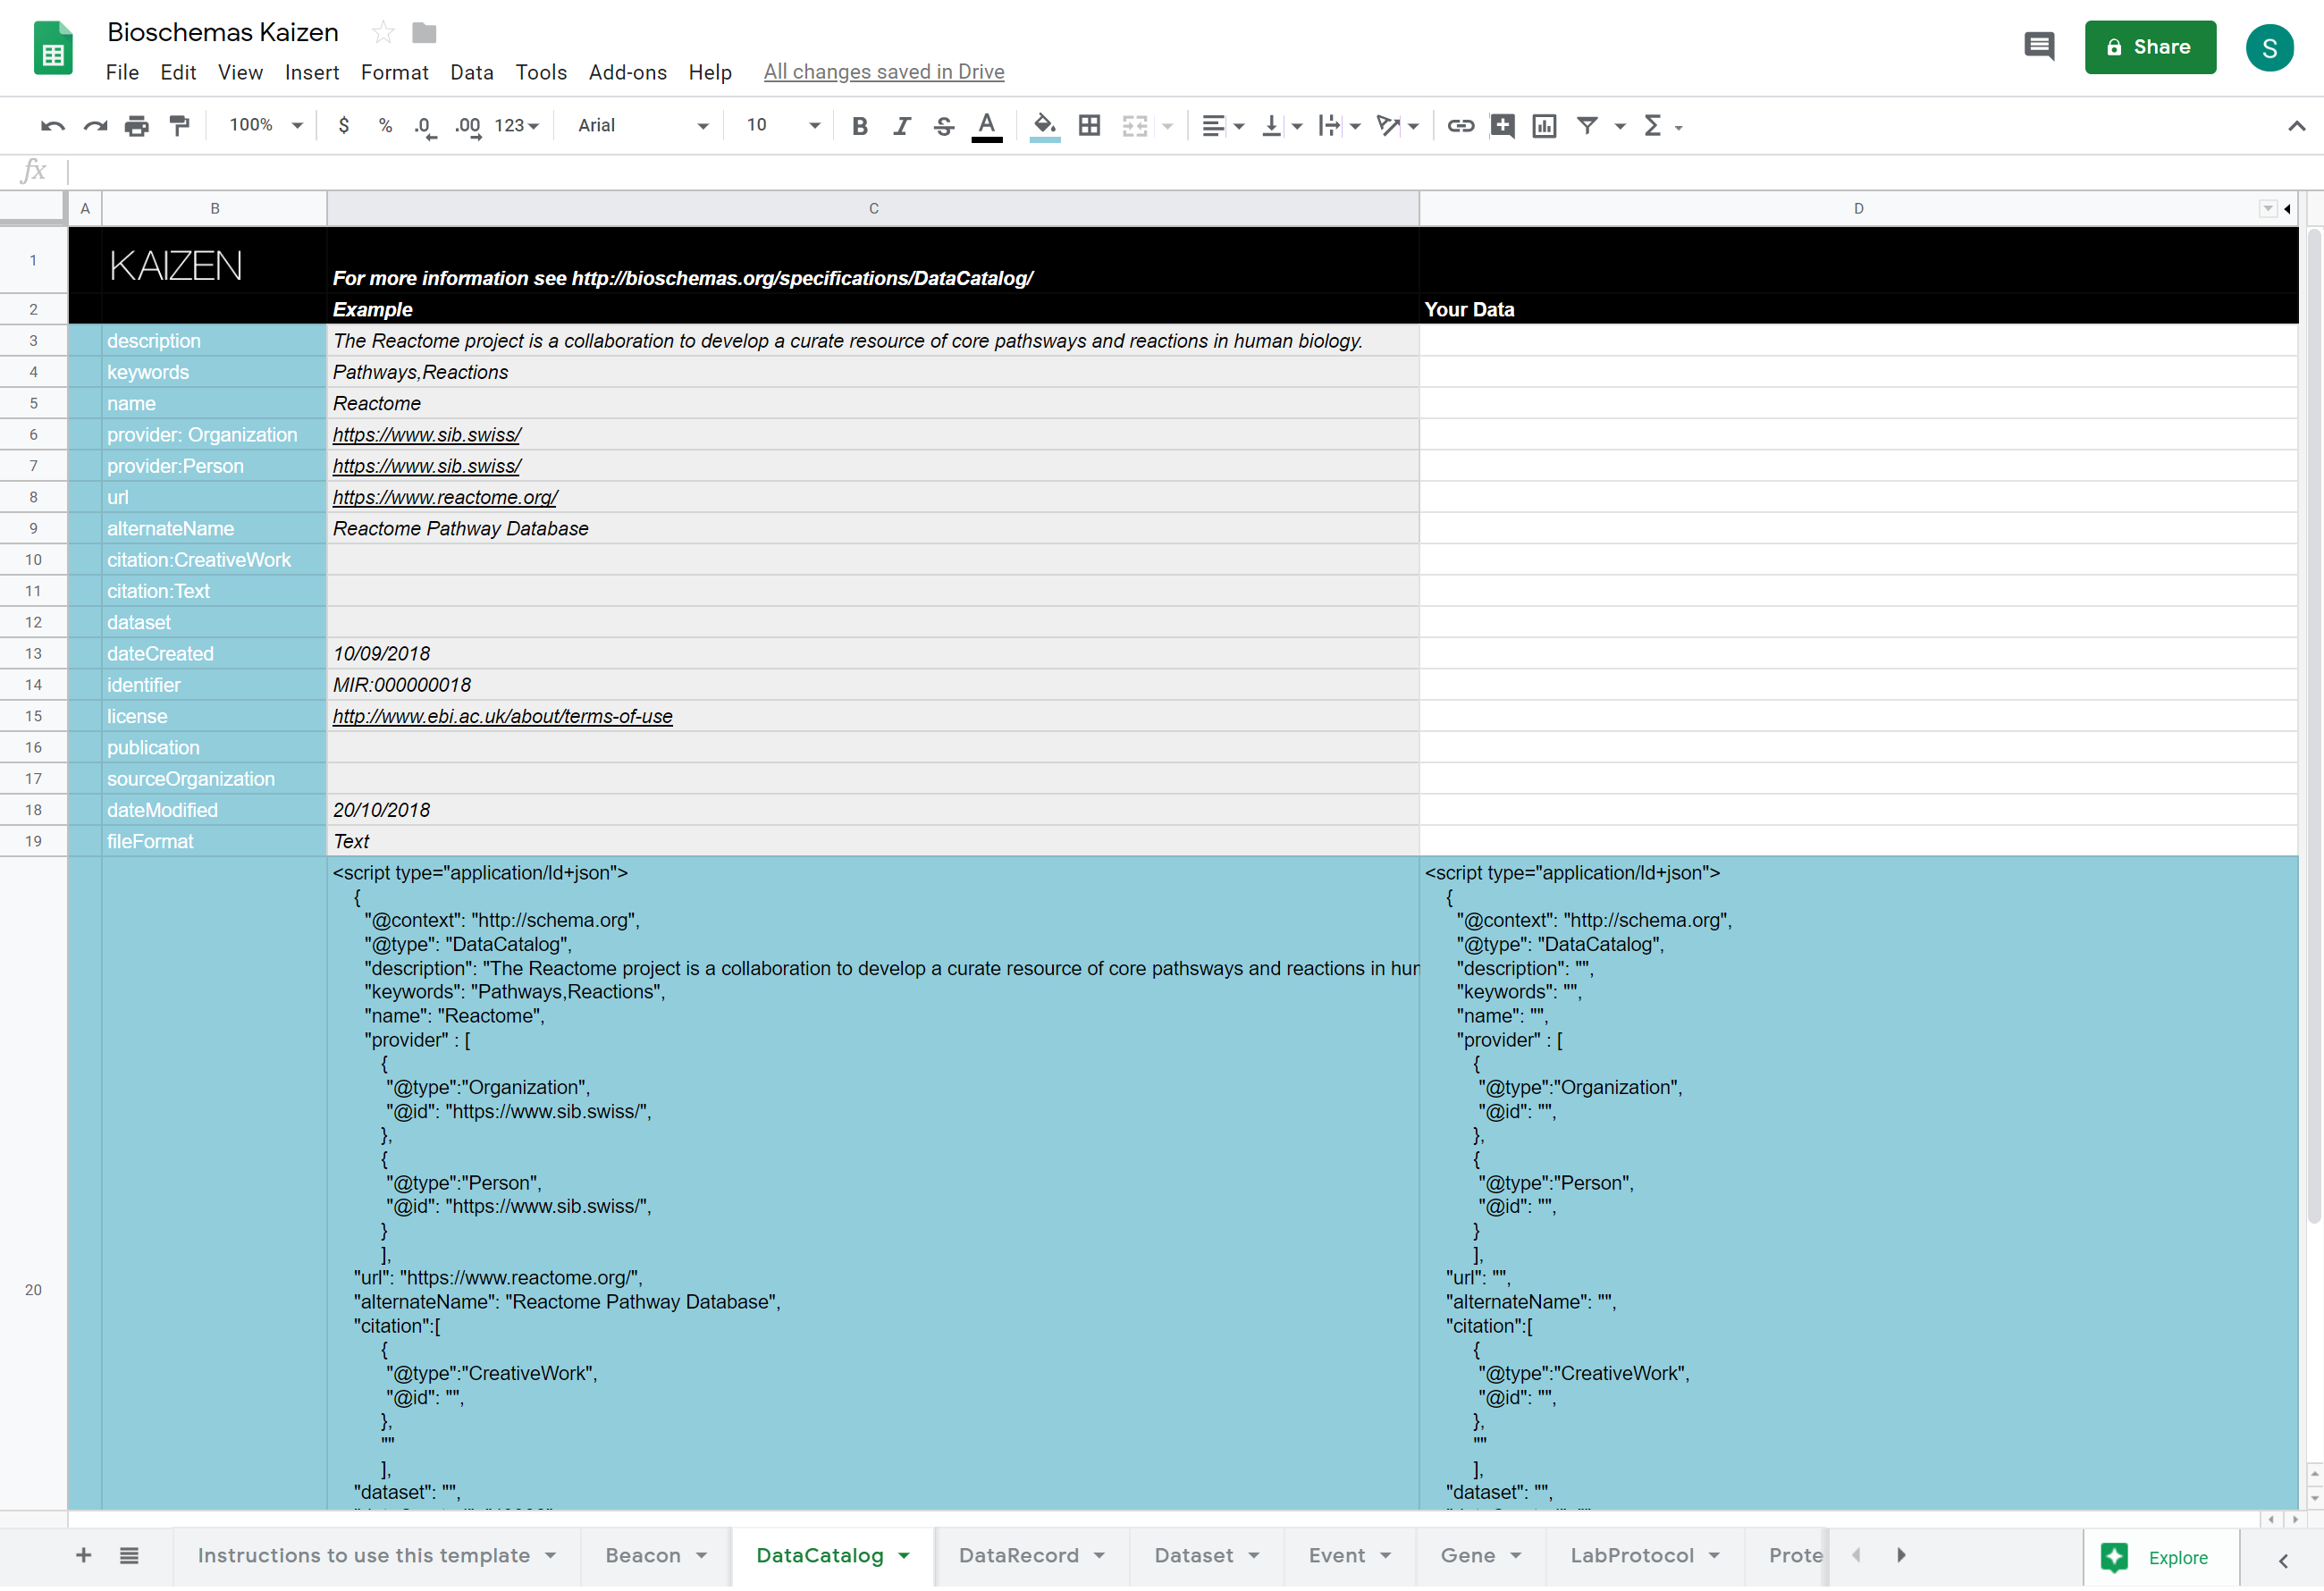
\includegraphics[scale=0.5]{images/system/BioschemasKaizen.PNG}
   \caption{Comparison System}
   \label{fig:comparisonSystem}
\end{figure}


datacatalog was created

examples given, no additional information, pointed to external source

\section{Maintainability}
After the successful completion of both the main and comparison system, the maintainability of each of the systems was compared to see how easy the systems were to keep up to date with the latest Bioschemas profiles.

For the main system, the webmaster of the system would simply have to re-run the scripting tool (See Section \ref{sec:scriptingtool}) to receive the updated files required for the web application. Once the files have been replaced with the newly generated files, the system will automatically have the latest Bioschemas profiles available to use.

On the other hand for the comparison system, the webmaster of the system would have to manually check and update each profile as there is currently no automated way of doing so. Additionally, as users create a local copy of the Google Sheet template, to receive the latest Bioschemas profiles the users have to check that they are using the latest version and download the newest version if available to keep up to date.


\section{Summary}
Although there were a few issues surrounding the generation and use of the JSON-Schema, the core functionality of the proposed system was successfully developed. A user can select which Bioschemas profile they wish to generate a markup for, then provide the data using the form with the help of descriptions, controlled vocabularies and examples. Once the form is filled out they can then generate JSON-LD, Microdata or RDFa to use on their web page. Furthermore, a second comparison system was implemented for the final usability evaluation and the maintainability of each of the system was compared.